% arara: pdflatex: { synctex: yes }
% arara: makeindex: { style: ctuthesis }
% arara: bibtex

% The class takes all the key=value arguments that \ctusetup does,
% and a couple more: draft and oneside
\documentclass[twoside]{ctuthesis}

\ctusetup{
	preprint = \ctuverlog,
	mainlanguage = english,
	titlelanguage = english,
%	mainlanguage = czech,
	otherlanguages = {slovak,english},
	title-czech = {Moje bakalářka se strašně, ale hrozně dlouhým předlouhým názvem},
	title-english = {Drone detection using neural networks from combined RGB camera and LiDAR data},
	subtitle-czech = {Cesta do tajů kdovíčeho},
%	subtitle-english = {Journey to the who-knows-what wondeland},
	doctype = B,
	faculty = F3,
	department-czech = {Katedra matematiky},
	department-english = {Department of Cybernetics},
	author = {Adam Škuta},
	supervisor = {Matouš Vrba},
	supervisor-address = {Ústav X, \\ Uliční 5, \\ Praha 99},
	supervisor-specialist = {Martin Saska},
	fieldofstudy-english = {Mathematical Engineering},
	subfieldofstudy-english = {Mathematical Modelling},
	fieldofstudy-czech = {Matematcké inženýrství},
	subfieldofstudy-czech = {Matematické modelování},
	keywords-czech = {slovo, klíč},
	keywords-english = {word, key},
	day = 10,
	month = 2,
	year = 2017,
	specification-file = {ctutest-zadani.pdf},
%	front-specification = true,
%	front-list-of-figures = false,
%	front-list-of-tables = false,
%	monochrome = true,
%	layout-short = true,
}

\ctuprocess

\addto\ctucaptionsczech{%
	\def\supervisorname{Vedoucí}%
	\def\subfieldofstudyname{Studijní program}%
}

\ctutemplateset{maketitle twocolumn default}{
	\begin{twocolumnfrontmatterpage}
		\ctutemplate{twocolumn.thanks}
		\ctutemplate{twocolumn.declaration}
		\ctutemplate{twocolumn.abstract.in.titlelanguage}
		\ctutemplate{twocolumn.abstract.in.secondlanguage}
		\ctutemplate{twocolumn.tableofcontents}
		\ctutemplate{twocolumn.listoffigures}
	\end{twocolumnfrontmatterpage}
}

% Theorem declarations, this is the reasonable default, anybody can do what they wish.
% If you prefer theorems in italics rather than slanted, use \theoremstyle{plainit}
\theoremstyle{plain}
\newtheorem{theorem}{Theorem}[chapter]
\newtheorem{corollary}[theorem]{Corollary}
\newtheorem{lemma}[theorem]{Lemma}
\newtheorem{proposition}[theorem]{Proposition}

\theoremstyle{definition}
\newtheorem{definition}[theorem]{Definition}
\newtheorem{example}[theorem]{Example}
\newtheorem{conjecture}[theorem]{Conjecture}

\theoremstyle{note}
\newtheorem*{remark*}{Remark}
\newtheorem{remark}[theorem]{Remark}

\setlength{\parskip}{5ex plus 0.2ex minus 0.2ex}
\graphicspath{{figures/}}

% Abstract in Czech
\begin{abstract-czech}
\end{abstract-czech}

% Abstract in English
\begin{abstract-english}
\end{abstract-english}

% Acknowledgements / Podekovani
\begin{thanks}
Děkuji ČVUT, že mi je tak dobrou \emph{alma mater}.
\end{thanks}

% Declaration / Prohlaseni
\begin{declaration}
Prohlašuji, že jsem předloženou práci vypracoval samostatně, a že jsem uvedl veškerou použitou literaturu.

V Praze, \ctufield{day}.~\monthinlanguage{title}~\ctufield{year}
\end{declaration}

% Only for testing purposes
\listfiles
\usepackage[pagewise]{lineno}
\usepackage{lipsum,blindtext}
\usepackage{mathrsfs} % provides \mathscr used in the ridiculous examples
\usepackage{todonotes}
\usepackage{amsmath}
\usepackage{xspace}
\usepackage{caption}
\usepackage{subcaption}
\usepackage{multirow}
\usepackage{hyperref}

\begin{document}

\maketitle
\chapter{Introduction}
In this thesis a drone detection using neural networks from combined RGB camera and LiDAR data is studied. With the recent development of drone technology, drones have become more readily available to public and could only be expected to rise in popularity in the future. Drone detection is an important problem to tackle when it comes to tasks such as interception of uncooperative drones \cite{cite:1} or localization of drones in swarm \cite{cite:2} \cite{cite:3}. Furthermore Light detection and ranging (LiDAR) sensors mounted on drones have been utilized \cite{cite:4} and provide a viable sensor option. Therefore fusing camera and LiDAR sensor could be used for more accurate localization.\\
\\
The goal of this thesis was to examine whether a usage of LiDAR data coupled with RGB images from camera is useful for the localization of drones in contrast to the usage of image data alone.The LiDAR and RGB camera were mounted on top of the observer drone, which took pictures and pointclouds of the target drone. All the measurements were taken inside a virtual environment, with a realistic drone and sensor simulation. The dataset was then processed and used as the input for training and testing a Convolutional neural network for the object detection. The preprocessing was as following:
\begin{itemize}
	\item Coordinate transformation for the non-matching coordinate systems,
	\item Projection of 3d points into a 2d image,
	\item Utilizing different processing methods on sparse LiDAR point cloud in order to make it more dense,
	\item Fusing RGB images and LiDAR data into RGBD images.
\end{itemize}
The output metrics were then compared with the RGB trained convolutional neural network metrics.
\begin{figure}[h]
	\centering
	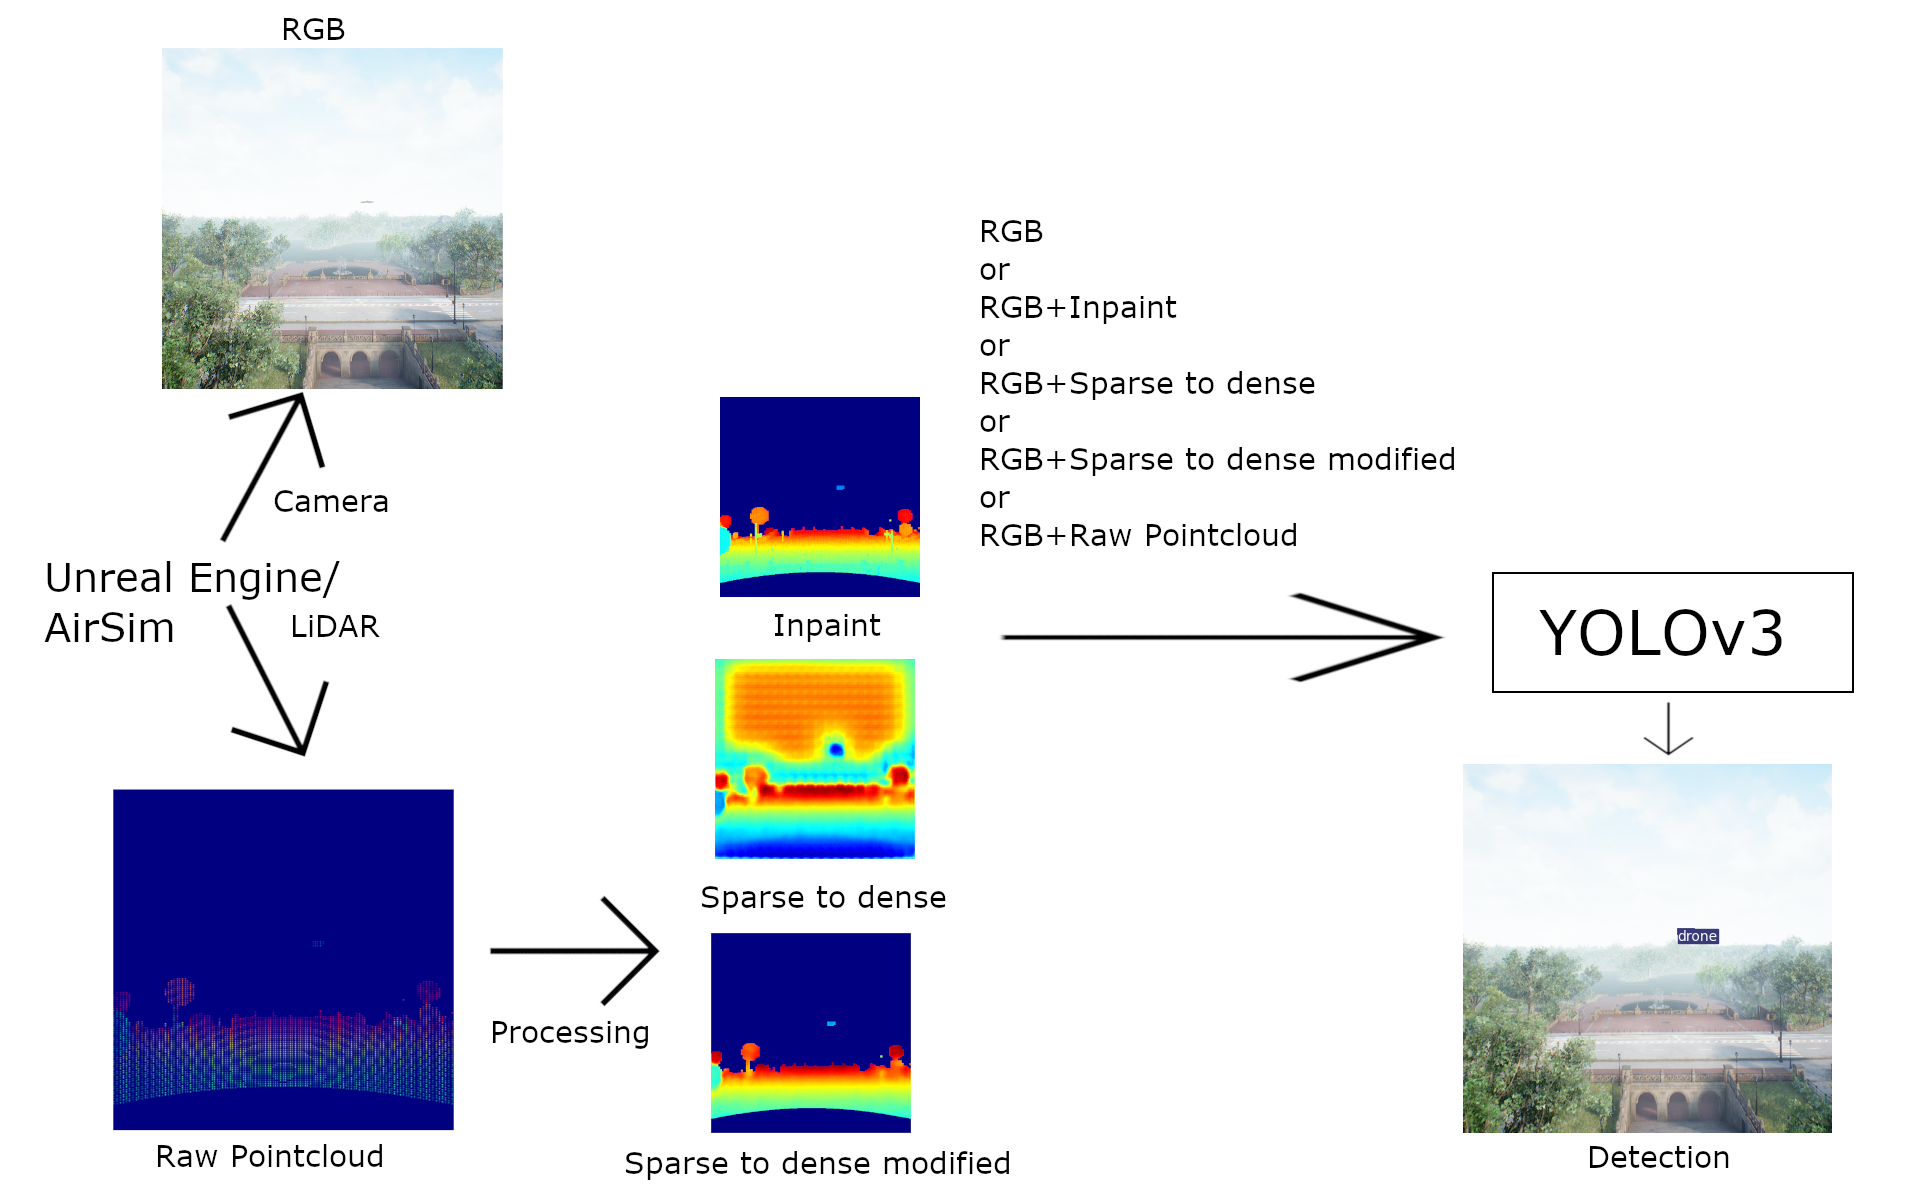
\includegraphics[width=\textwidth]{intro_schemav2.png}
	\caption{Schema of the process.}
\end{figure}
\section{Related Work}
Solving the problem of drone detection has been tackled in different ways. The main difference between them is the choice of sensor or sensors utilized. 
\chapter{Methodolology}
In this chapter various methods used in this thesis are discussed. A video game engine Unreal Engine\footnote{\url{https://www.unrealengine.com}}paired with plugin AirSim\footnote{\url{https://microsoft.github.io/AirSim/}} was used for simulating real-life environments and for generating the dataset. An image inpainting technique was used as an option for transforming sparse LiDAR pointcloud into a dense one. A convolutional neural network was used in two problems in the thesis. First one was on a sparse LiDAR pointcloud generating more points and therefore making it more dense. Second one was used for object, in this case drone, detection using RGB and RGBD data as the input.
\section{Sparse to dense} \label{s2d}
Sparse to dense is a Convolutional neural network written in PyTorch. \cite{ma2018sparsetodense} It predicts the depth measurements from sparse depth dataset. The size of the network is modifiable and can be chosen as training parameters.
\begin{figure}[h]
	\caption{Example of different network architectures available. Taken from \cite{ma2018sparsetodense}.}
	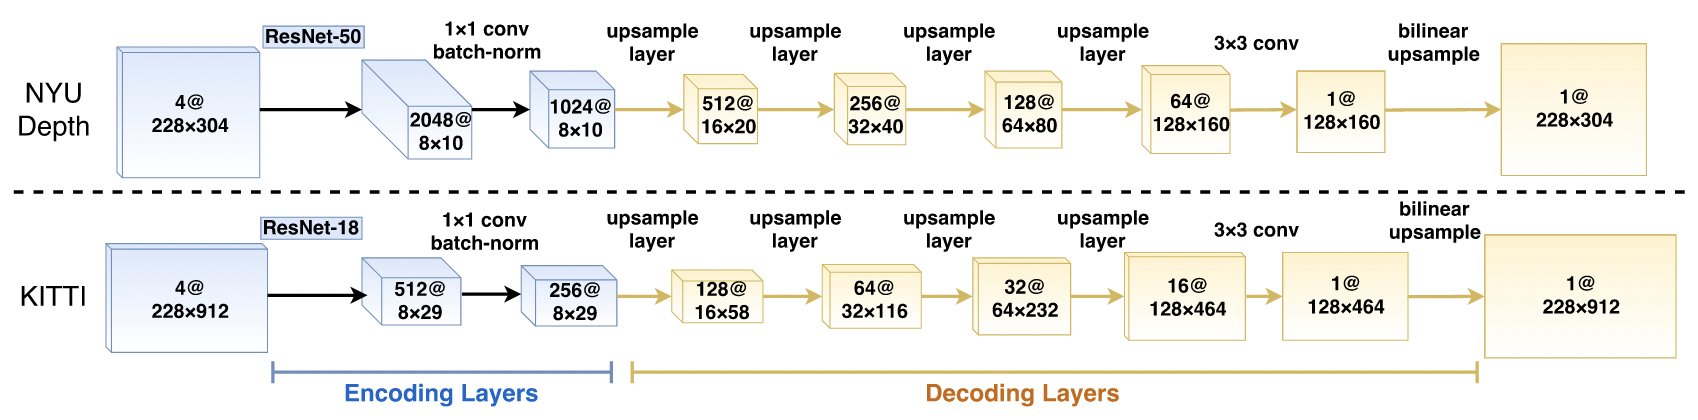
\includegraphics[width=\textwidth]{sparse2dense.png}
	\centering
\end{figure}
For the encoding and therefore input layers a ResNet-50 or ResNet-18 can be chosen, depending on the size of the input image for memory constraints. The decoding layers consist of 4 upsampling layers and a deconvolutional layer with either stride 2 or 3 or uprojection layer or upconvolutional layer as a choice for training. The default loss function is least absolute deviations also known as $L_1$ error:
\begin{equation}
	L_1=\sum_{i=1}^{n}|y_{true}-y_{predicted}|,
\end{equation}
where:
\begin{itemize}
	\item n is batch size,
	\item $y_{true}$ are real depth values,
	\item $y_{predicted}$ are predicted depth values.
\end{itemize}
The input to the network are RGBD images and the output is a depth map with the same dimensions as input. The depth input $D$ is sampled from the ground truth depth map $D^*$ with the following formula:
\begin{equation}
	D(i,j)=\begin{cases}
		D^*(i,j),&\text{with probability}\ p,\\
		0,&\text{otherwise},
	\end{cases}
\end{equation}
where:
\begin{itemize}
	\item $i,j$ are coordinates of the input image,
	\item $p=\frac{m}{n}$, where $m$ number of depth samples to be chosen at the start of training and $n$ is the total amount of available depth samples.
\end{itemize}
During training several input data augmentations take place. These augmentations include:
\begin{itemize}
	\item Scaling the input image by a random number $s\in[1,1.5]$,
	\item Rotating the input image by a random degree $r\in[-5,5]$,
	\item Scaling the brightness, contrast and saturation of the RGB component of the image by a random number $k\in[0.6,1.4]$,
	\item Normalizing the RGB component of the image,
	\item Flipping the image horizontally with a 50\% chance.
\end{itemize}
The output of the network is a dense depth image with the dimensions of the input. Every pixel contains predicted depth measurement in meters. The output of the Sparse to Dense network will be used for further training later.
\section{YOLOv3}
\todo{citations}
You only look once (YOLO) is a convolutional neural network model used mainly for object detection and recognition\cite{redmon2016look}. The main advantage is its simplicity in comparison to similar convolutional neural networks, resulting in faster detection speeds. It belongs to the state of the art convolutional neural networks for object detection and recognition. The version used in this work is the third version YOLOv3\cite{redmon2018yolov3}. The backbone called Darknet53 consists of 53 convolutional layers. The original detector consists of 3 detection layers each responsible for detecting objects of various sizes. 
\begin{figure}[h]
	\caption{YOLOv3 network architecture. Taken from \cite{kathuria_2018}}
	\centering
	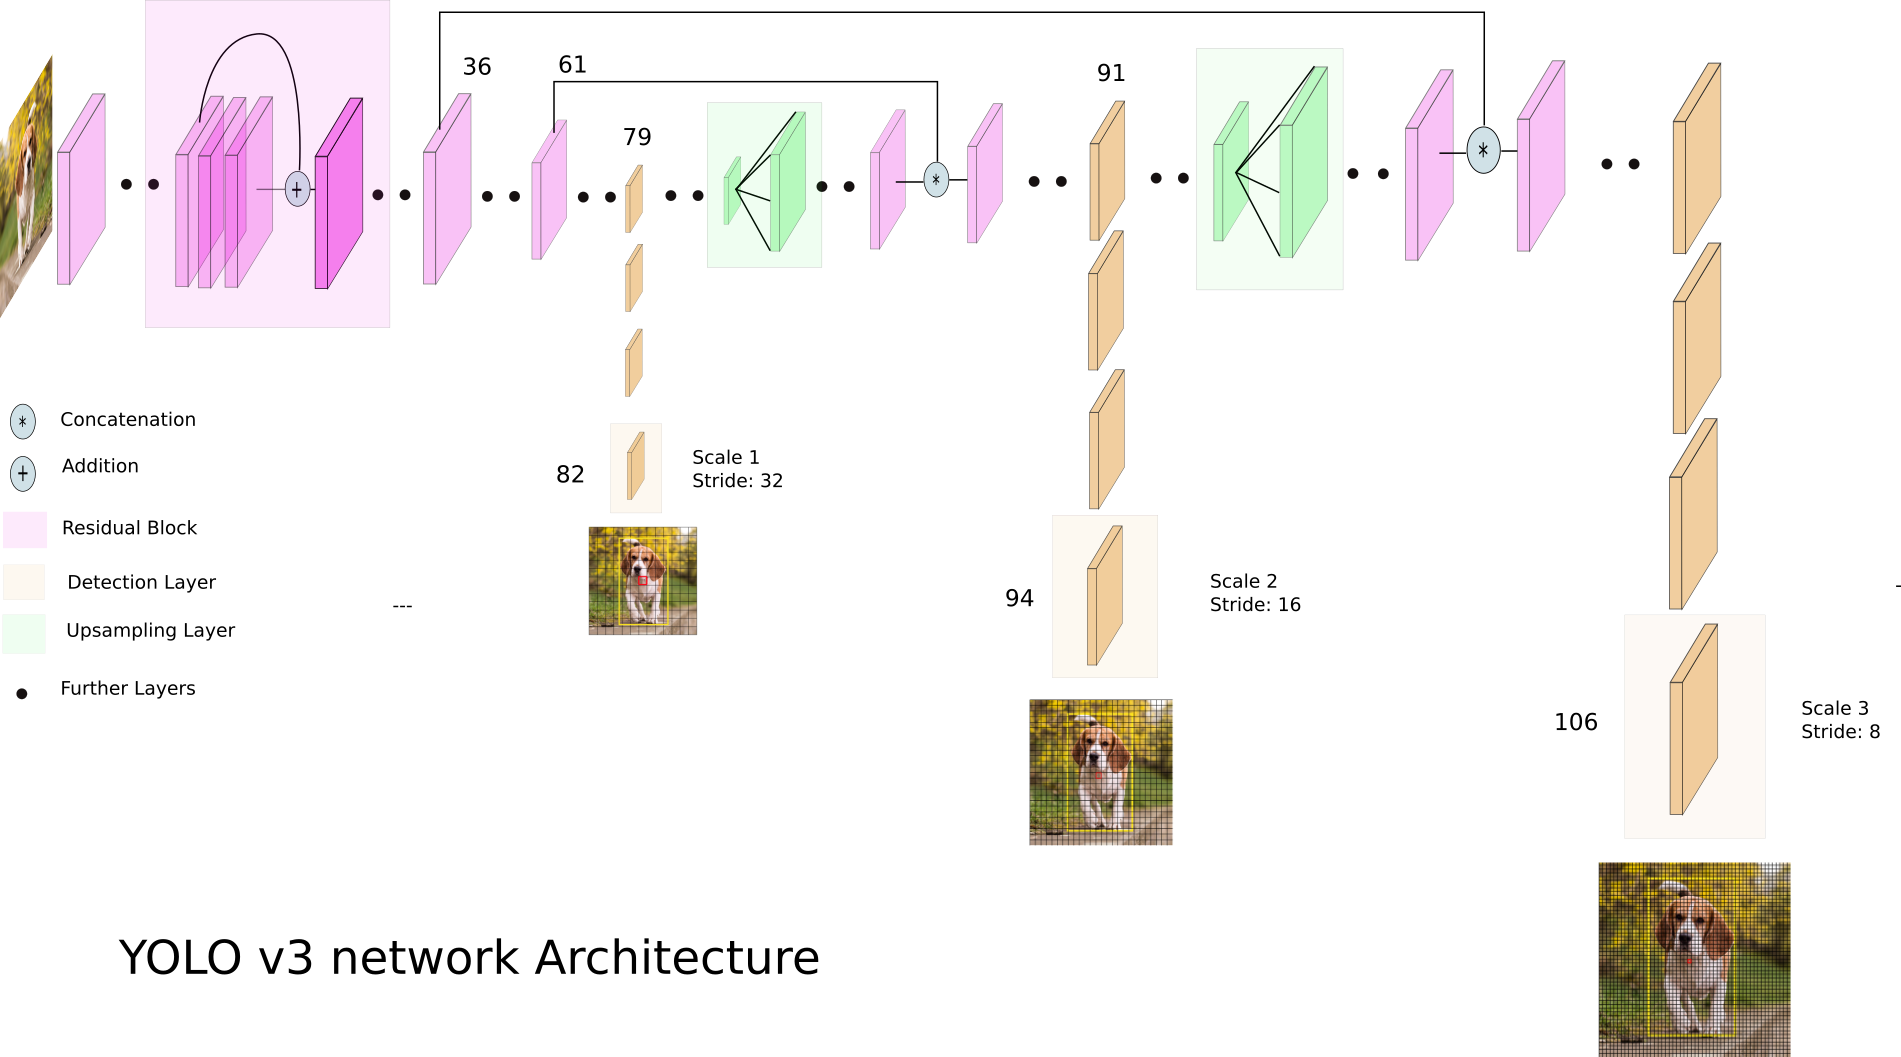
\includegraphics[width=\textwidth]{yolov3_model.png}
\end{figure}
At each detection layer, the image is divided into multiple grid cells, where each grid cell detects three bounding boxes. YOLOv3 takes $n$-channel images as the input. Each of the detection layers outputs three bounding boxes for each of the cell. The content of one bounding box is as following:
\begin{itemize}
	\item $t_x, t_y, t_w, t_h$ are bounding box co-ordinates,
	\item $p_O$ is objectness score,
	\item $p_c$ is class score for each class in the dataset.
\end{itemize}
The bounding box $t_x$ and $t_y$ coordinates are relative to the upper-left corner of its respective cell, while $t_w$ and $t_h$ are relative to one of the anchors. Anchors are pre-defined default bounding box sizes and can be modified before training. To transform these bounding box coordinates to be relative to the image following transformation is applied:
\begin{equation}\label{bbox}
	\begin{aligned}
		b_x&=\sigma(t_x)+c_x,\\
		b_y&=\sigma(t_y)+c_y,\\
		b_w&=p_{w}e^{t_w},\\
		b_h&=p_{w}e^{t_h},
	\end{aligned}
\end{equation}
where:
\begin{itemize}
	\item $\sigma(x)$ is a sigmoid function,
	\item $c_x, c_y$ are grid cells offsets from the top left corner of the image,
	\item $p_w, p_h$ are anchors width and height respectively,
	\item $b_x, b_y, b_w, b_h$ are bounding box coordinates relative to the image size.
\end{itemize}
The loss function used during the training is sum squared error loss or $L_2$ error described as follows:
\begin{equation}
	L_2=\sum_{i=1}^{n}(\mathbf{\hat{t}}-\mathbf{t})^2,
\end{equation}
where:
\begin{itemize}
	\item $n$ is batch size,
	\item $\mathbf{\hat{t}}$ is vector of predicted bounding box co-ordinates,
	\item $\mathbf{t}$ is vector of ground truth bounding box coordinates which can be obtained by inverting transformation in \ref{bbox}.
\end{itemize}
\section{Image inpainting method based on the Fast Marching Method} \label{inpainting}
Image inpainting is a method used for reconstructing missing values in the image. A one such method based on \cite{cite:5} called Image inpainting method based in the Fast Marching Method is presented in this section. A grayscale image is used for simplification purposes.\\
\\
The grayscale value of a pixel to be inpainted is determined by the known neighboring pixel values. To compute grayscale value from one close pixel a following formula is used:
\begin{equation} \label{eq:1}
	I_q(p)=I(q)+\nabla I(q)(p-q),
\end{equation}
where:
\begin{itemize}
	\item $q$ are pixel co-ordinates with known grayscale value,
	\item $p$ are pixel co-ordinates with unknown grayscale value,
	\item $I(x)$ is a grayscale value at pixel co-ordinates $x$,
	\item $\nabla I(x)$ is a gradient value at pixel co-ordinates $x$.
\end{itemize}
\begin{figure}[h]
	\centering
	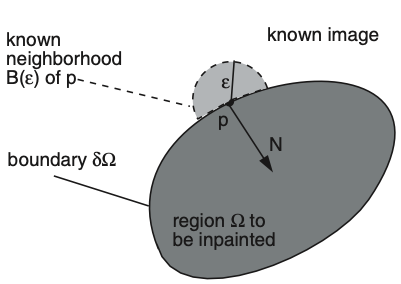
\includegraphics[width=10cm]{inpaint_principle.png}
	\caption{Inpainting principle. Image from: \cite{cite:5}}
\end{figure}
To get a final value for the unknown pixel the Equation \ref{eq:1} is applied on all known pixels in a specified region $B_{\varepsilon}(p)$ from the unknown pixel. The function is as following:
\begin{equation}\label{inpaint_eq}
	I(p)=\frac{\sum_{q\in B_{\varepsilon}(p)}w(p,q)I_q(p)}{\sum_{q\in B_{\varepsilon}(p)}w(p,q)},
\end{equation}
where $w(p,q)$ is a weighting function designed for propagating sharpness of the image and is obtained as the product of the following equations:
\begin{equation}
	\begin{aligned}
		dir(p,q)&=\frac{p-q}{||p-q||}N(p),\\
		dst(p,q)&=\frac{1}{||p-q||^2},\\
		lev(p,q)&=\frac{1}{1+|T(p)-T(q)|},
	\end{aligned}
\end{equation}
where,
\begin{itemize}
	\item $N(x)$ is a normal direction of the boundary to be inpainted at pixel co-ordinates $x$,
	\item $T(x)$ is distance of pixel $x$ to the inpainting boundary.
\end{itemize}
The equation \ref{inpaint_eq} is iteratively applied to all pixels on the inpainting boundary, and advances inside the region to be inpainted until the whole region has been filled. This is implemented via Fast Marching Method algorithm.
\begin{figure}[h!]
	\caption{Example of the inpainting technique. Image from: \cite{cite:5}}
	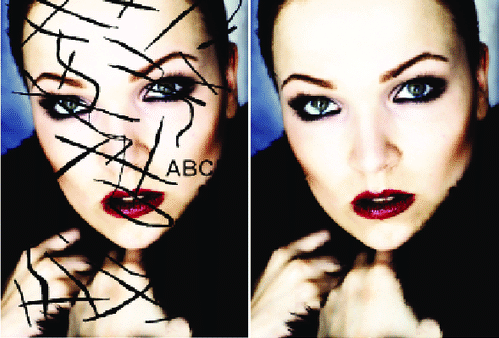
\includegraphics[width=10cm]{inpaint_example.png}
	\centering
\end{figure}
\section{Coordinate systems}
In order to correctly label the data for training, a position of the target drone in relation to the sensor mounted on the observer drone is required. The AirSim API returns the position of each drone in respect to their starting points. The starting point is a point where the drone spawns in the map. Therefore a transformation from the starting point of the target drone to the camera mounted on the observer is required. This transformation is written as follows:
\begin{equation}
	\textbf{T}=\textbf{T}_{o}^{c}\textbf{T}_{os}^{o}\textbf{T}_{ts}^{os},
\end{equation}
where:
\begin{itemize}
	\item $\textbf{T}_{ts}^{os}$ is transformation from the starting point of the target drone to the starting point of the observer drone,
	\item $\textbf{T}_{os}^{o}$ is transformation from the starting point of the  to the body of the first drone,
	\item $\textbf{T}_{o}^{c}$ is transformation from the body of the first drone to the cameras coordinate system.
\end{itemize}
\begin{figure}[h]
	\centering
	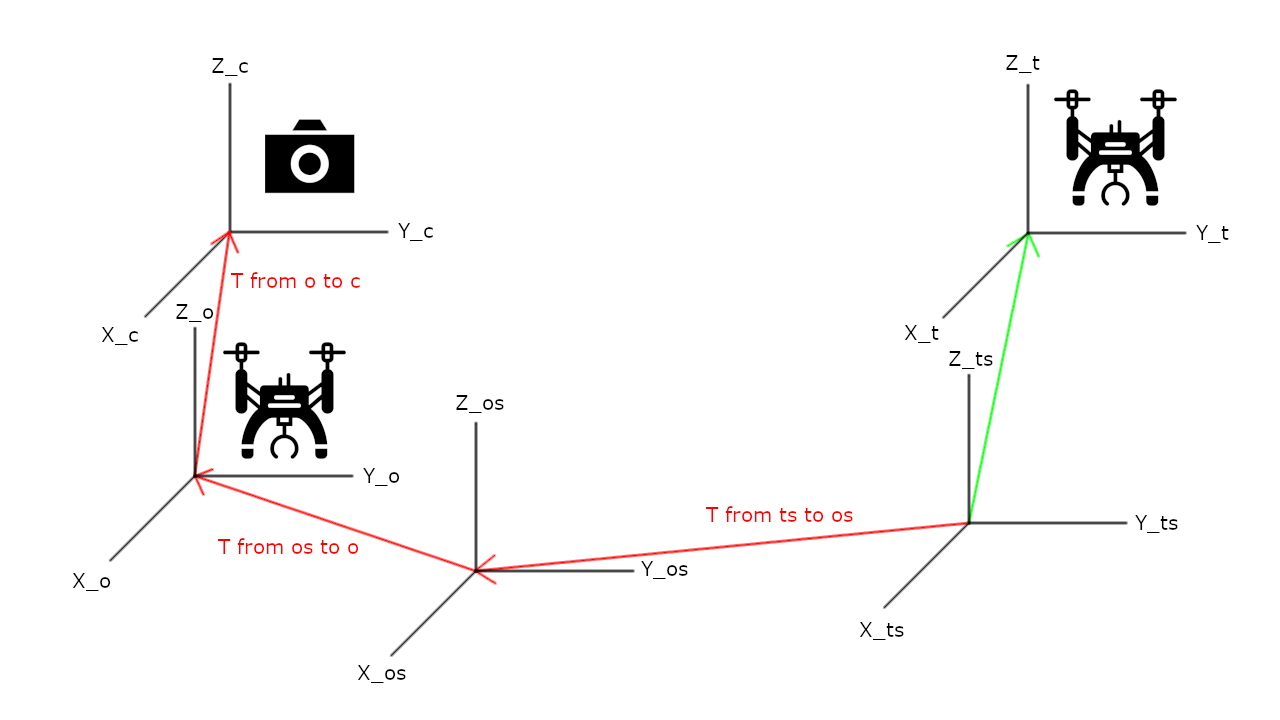
\includegraphics[width=\textwidth]{coord_schema.png}
	\caption{Visualization of transformation.}
\end{figure}
Transformation matrix $\textbf{T}$ is generally be described as follows:
\begin{equation}
	\textbf{T}=\begin{bmatrix}
		\textbf{R} & \textbf{p}\\
		\textbf{0}^T & 1
	\end{bmatrix},
\end{equation}
where:
\begin{itemize}
	\item $\textbf{R}$ is a 3x3 rotation matrix,
	\item $\textbf{p}$ is a 3x1 translation column vector,
	\item $\textbf{0}^T$ is a 1x3 row vector of zeros.
\end{itemize}
\section{Camera Model}
For the creation of the bounding boxes used for training and for processing raw data from LiDAR sensor a transformation from coordinate system of the camera to the pixel values of the image needs to be defined. For this task a pinhole camera model is used.
\begin{figure}[h]
	\centering
	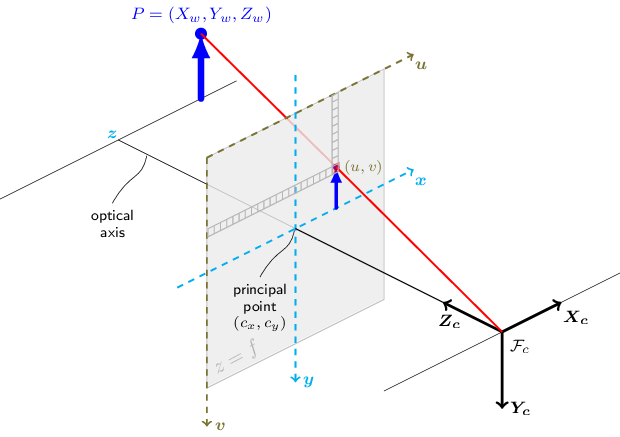
\includegraphics[width=\textwidth]{pinhole_camera_model.png}
	\caption{Pinhole camera model. Image from \cite{opencv}.}
\end{figure}\\
The transformation is then defined as follows:
\begin{equation} \label{eq:2}
	\begin{bmatrix}
		u\\
		v
	\end{bmatrix}=
	\begin{bmatrix}
		f\frac{X_c}{Z_c}+c_x\\
		f\frac{Y_c}{Z_c}+c_y
	\end{bmatrix},
\end{equation}
where:
\begin{itemize}
	\item $u$ and $v$ are pixel coordinate values on the image,
	\item $X_c$,$Y_c$,$Z_c$ are coordinate values of a point in the coordinate system of the camera,
	\item $f$ is focal length of the camera,
	\item $c_x$,$c_y$ are offsets on the image plane.
\end{itemize}
In order to transform the point from world coordinates $X_w,Y_w,Z_w$ to the coordinate system of the camera a following transformation needs to be applied:
\begin{equation}
	\begin{bmatrix}
		X_c\\
		Y_c\\
		Z_c\\
		1
	\end{bmatrix}=
	\begin{bmatrix}
		0 & 1 & 0 & 0\\
		0 & 0 & 1 & 0\\
		1 & 0 & 0 & 0\\
		0 & 0 & 0 & 1\\
	\end{bmatrix}
	\begin{bmatrix}
		X_w\\
		Y_w\\
		Z_w\\
		1
	\end{bmatrix}
\end{equation}
Pinhole camera model is only idealization of a real life camera and no lens distortion needs to be considered. The AirSim simulator simulates pinhole camera so no other processing needs to be done.
\section{Dataset}
The dataset for this work can be generated in two ways. The first is real-life drone shots mixed with point clouds from LiDAR mounted on top of a drone. The second is generating a dataset using a realistic virtual environment where a drone, camera and LiDAR are being emulated very close to their real-life counterparts. An advantage to this approach is that a great variety of environments can be chosen a lot of them often inaccessible otherwise (power plant, airport, snowy mountains out of season etc.). Therefore this approach was chosen for the task.
\subsection{Unreal Engine}
Unreal Engine is a software tool used for creating realistic 3d environments, most often used as a video game engine. It is written in C++ and open-source supporting a variety of pre-built environments and assets. For this work three different environments were used for the creation of the dataset:
\begin{itemize}
	\item City Park Environment Collection (2256 samples taken),
	\item Automotive Winter Scene (1813 samples taken),
	\item Downtown West Modular Pack(1120 samples taken).
\end{itemize}
\begin{figure}[h]
	\centering
	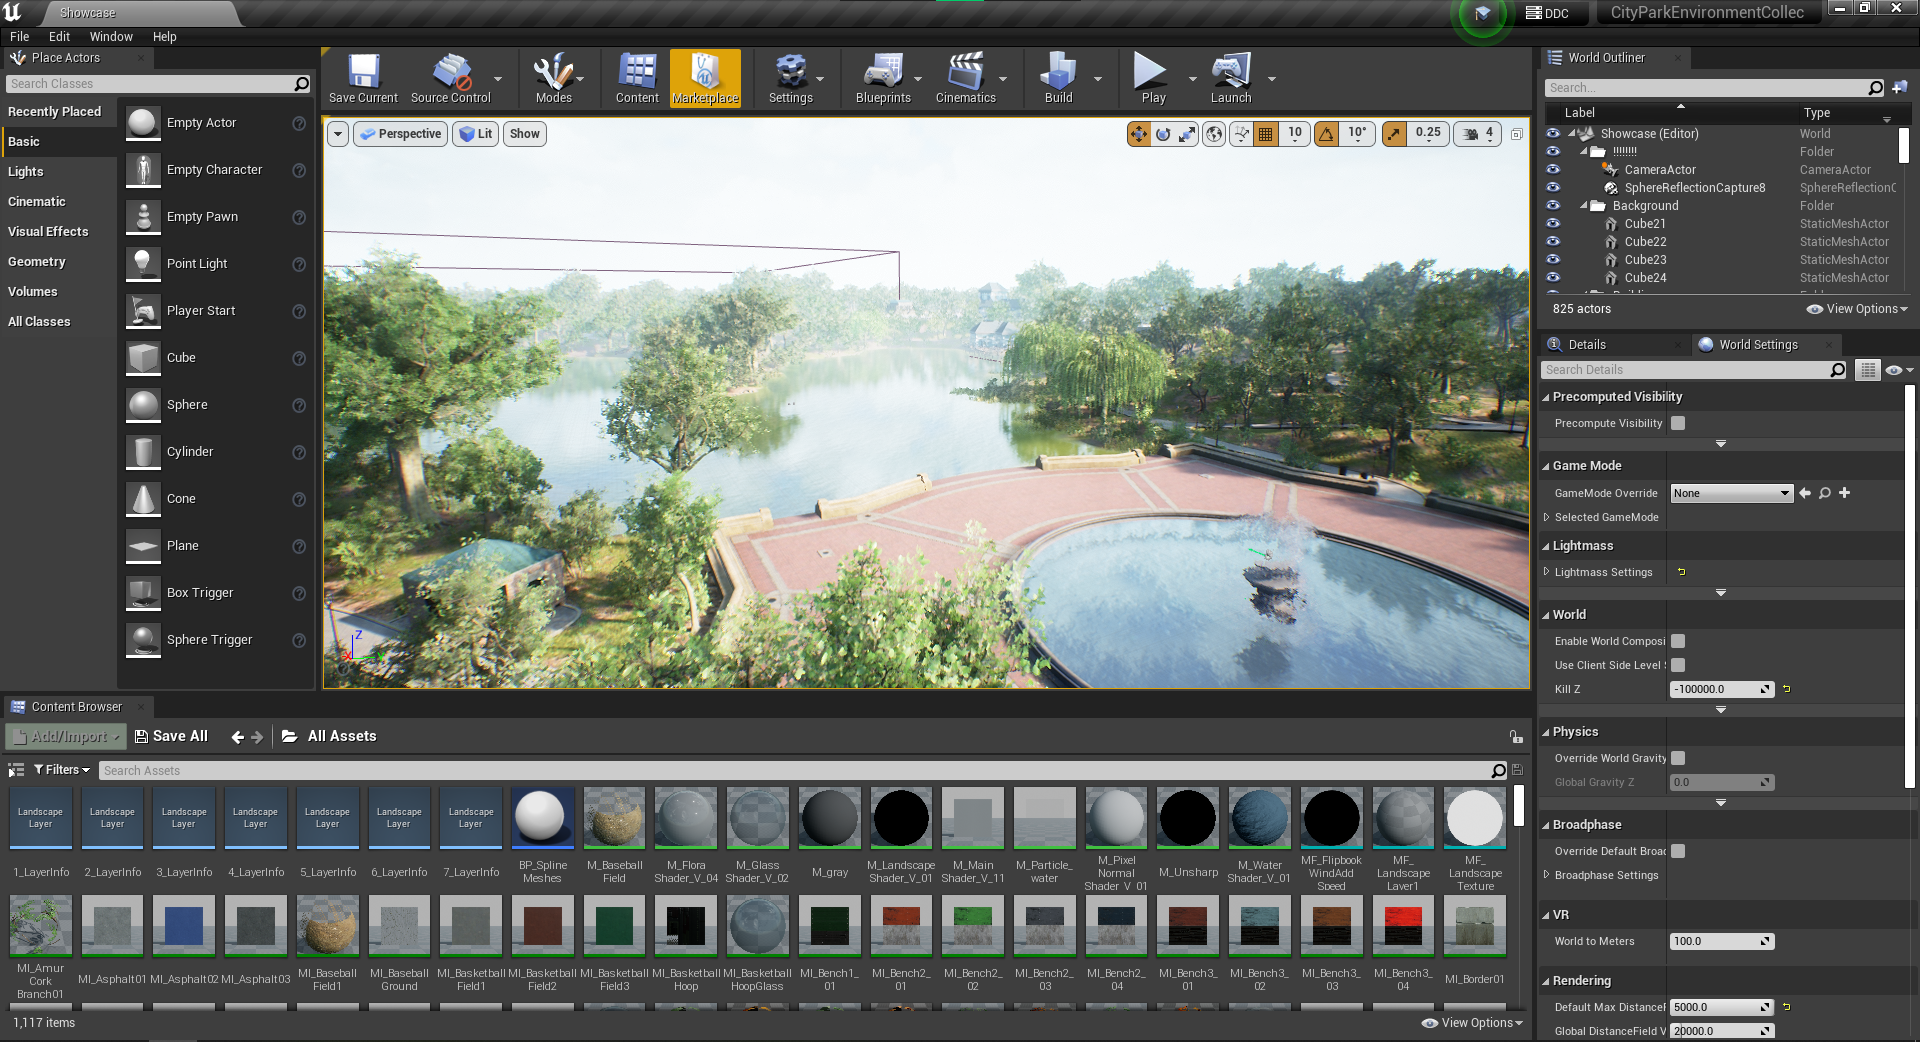
\includegraphics[width=\textwidth]{unreal_ui.png}
	\caption{Unreal Engine user interface.}
\end{figure}
Together 5320 pictures and labels were generated using two drones. Observer drone was equipped with RGB camera and LiDAR sensor and was responsible for taking the pictures and pointclouds from LiDAR. The target drone was used as a model for drone detection.
\subsection{AirSim}
Open-source plugin for Unreal Engine called AirSim was used for the generation of the dataset. It simulates realistic flight motions of drones as well as seven types of sensors, including RGB camera and LiDAR used for this task. AirSim supports both a C++ API as well as Python API, latter which was used for controlling the motion and capturing the dataset. Location of the second drone was generated through API call, which produces a location of the drone in global coordinate system of the map, which is later transformed to the local coordinates of the first drone carrying the LiDAR and RGB sensors using Equation \ref{eq:2}. The capturing drone traveled on each map on a 3D cube grid.
\begin{figure}
	\centering
	\begin{subfigure}[b]{0.3\textwidth}
		\centering
		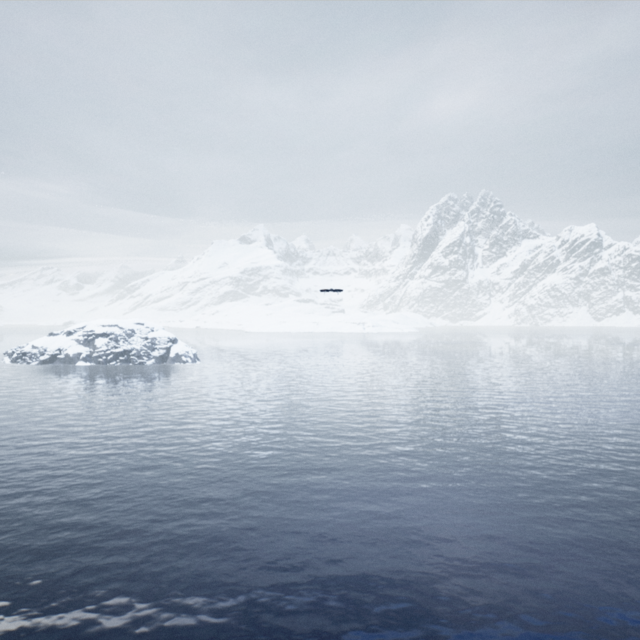
\includegraphics[width=\textwidth]{snow_rgb.png}
		\caption{Snow Environment.}
	\end{subfigure}
	\hfill
	\begin{subfigure}[b]{0.3\textwidth}
		\centering
		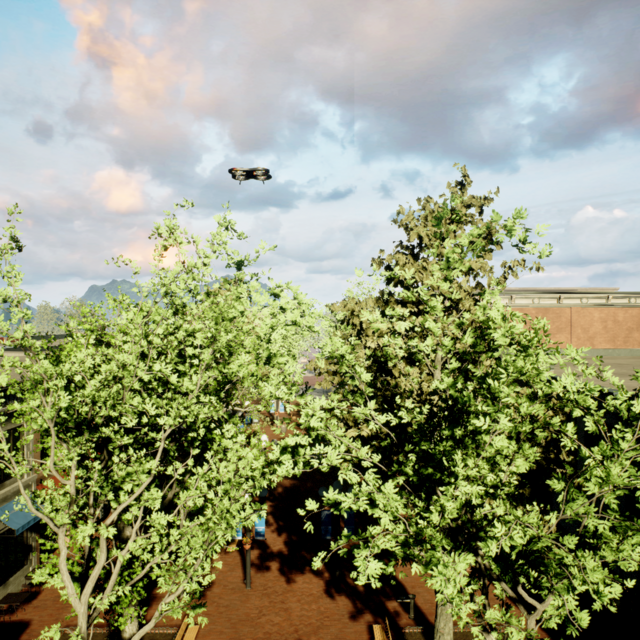
\includegraphics[width=\textwidth]{city_rgb.png}
		\caption{City Environment.}
	\end{subfigure}
	\hfill
	\begin{subfigure}[b]{0.3\textwidth}
		\centering
		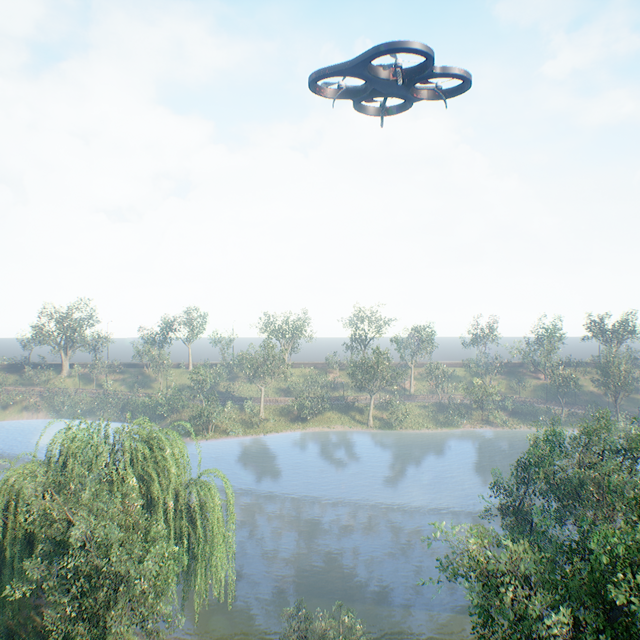
\includegraphics[width=\textwidth]{park_rgb.png}
		\caption{Park Environment.}
	\end{subfigure}
	\caption{Sample photos from each environment.}
\end{figure}
\section{Training}
For the training purposes 5320 samples were taken using AirSim simulator. Each sample consists of:
\begin{itemize}
	\item 640x640 RGB image from the camera,
	\item 640x640 sparse depth image from the LiDAR sensor,
	\item Label file containing ground truth bounding boxes co-ordinates.
\end{itemize}
This dataset was split into 3662 training, 407 validation, 1251 testing samples.
\subsection{Sparse to Dense}
The data were trained using Sparse to Dense neural network to receive dense depth image. The training was done for 15 epochs using batch size of 8. The backbone was Resnet18 and decoder was set to Deconv3 as described in \autoref{s2d}. The network was pretrained on Kitti\footnote{\url{http://www.cvlibs.net/datasets/kitti/}} dataset.
\begin{figure}
	\centering
	\begin{subfigure}[b]{0.4\textwidth}
		\centering
		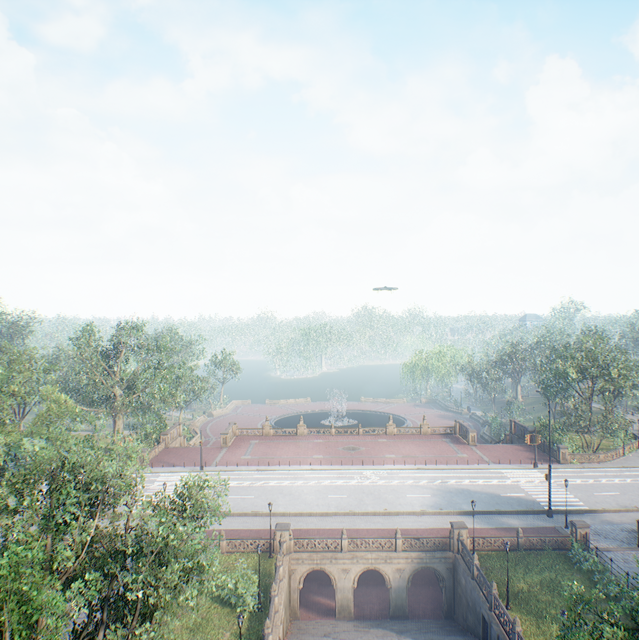
\includegraphics[width=\textwidth]{s2d_input.png}
		\caption{Input image.}
	\end{subfigure}
	\hfill
	\begin{subfigure}[b]{0.4\textwidth}
		\centering
		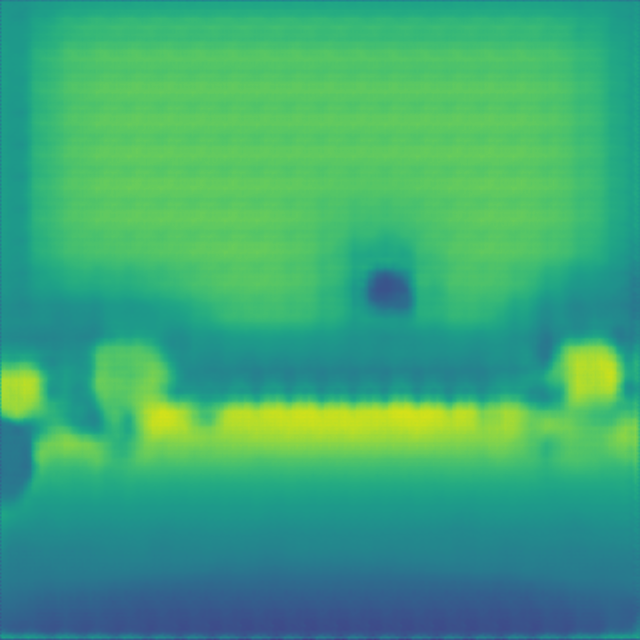
\includegraphics[width=\textwidth]{s2d_output.png}
		\caption{Output depth map.}
	\end{subfigure}
	\hfill
	\begin{subfigure}[b]{0.4\textwidth}
		\centering
		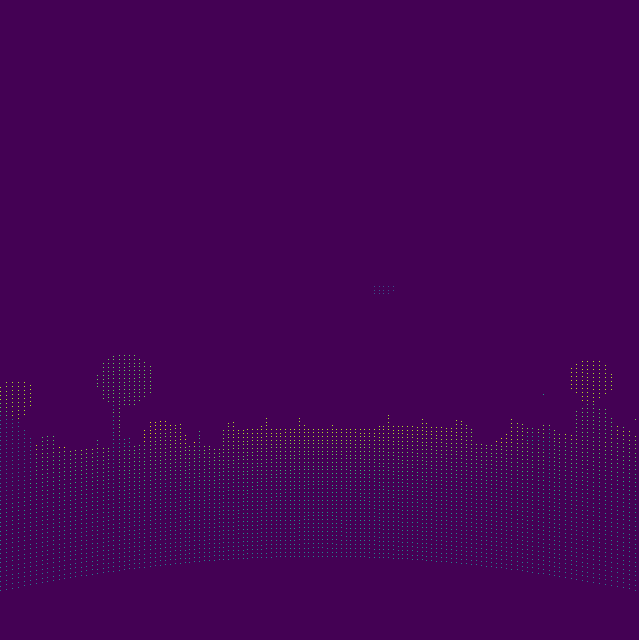
\includegraphics[width=\textwidth]{s2d_all.png}
		\caption{All pointcloud points.}
	\end{subfigure}
	\hfill
	\begin{subfigure}[b]{0.4\textwidth}
		\centering
		
\includegraphics[width=\textwidth]{s2d_select.png}
		\caption{Selected pointcloud points.}
	\end{subfigure}
	\caption{Sparse to dense training.}
\end{figure}
A processing algorithm was applied to the output depth map, further filtering points that were not in vicinity of the ground truth depth points. Both filtered and unfiltered depth maps were used for further training and testing to clarify their overall impact.
\begin{figure}[h!]
	\centering
	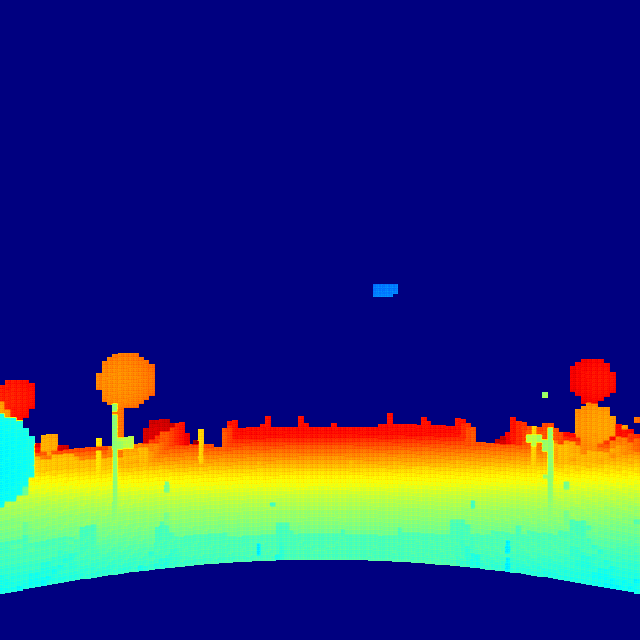
\includegraphics[width=5cm]{sparse2dense_filter.png}
	\caption{Applied filter on Sparse to dense output.}
\end{figure}
\subsection{Image inpainting}
An alternative algorithm for making sparse pointcloud into dense one was applied as well. The function is provided in OpenCV Python library. The input into the function was a sparse depth image, same as for the Sparse to dense network except the RGB part. The algorithm introduced in \ref{inpainting} was used with the radius of 1 pixel. The results were processed with the same filtering method as for the results of Sparse to dense method. For further training only the filtered depth map was used.
\begin{figure}[h]
	\centering
	\begin{subfigure}[b]{0.3\textwidth}
		\centering
		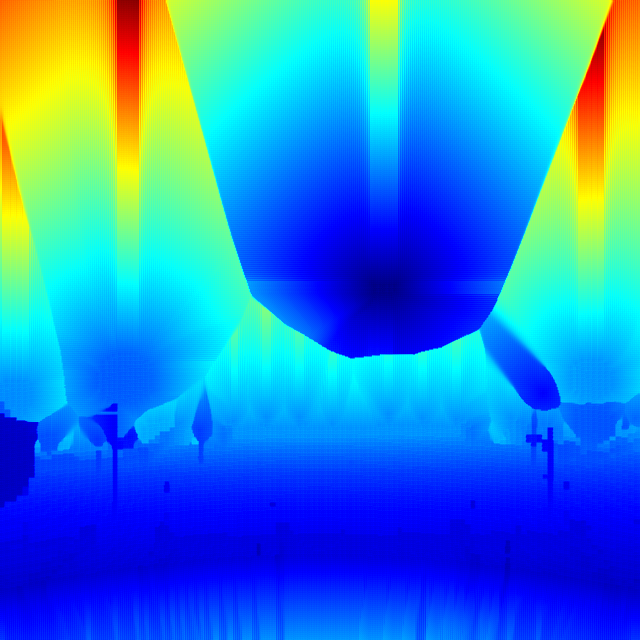
\includegraphics[width=\textwidth]{raw_inpaint.png}
		\caption{Non filtered result.}
	\end{subfigure}
	\hfill
	\begin{subfigure}[b]{0.3\textwidth}
		\centering
		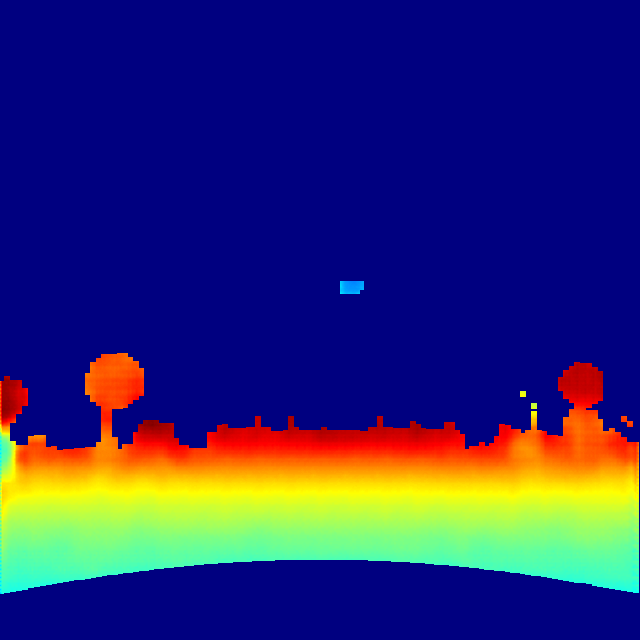
\includegraphics[width=\textwidth]{inpaint.png}
		\caption{Filtered result.}
	\end{subfigure}
	\caption{Inpaint results.}
\end{figure}
\subsection{YOLOv3}
Multiple different options of input to the YOLOv3 networks were applied. These include:
\begin{itemize}
	\item Concatenating the direct output of Sparse to dense neural network with the RGB images creating a RGBD image,
	\item Concatenating the modified Sparse to dense output with the RGB images creating RGBD image,
	\item Using OpenCV library to directly impaint the sparse depth image,
	\item Concatenating raw LiDAR pointcloud to the RGB image
	\item Using only the RGB image skipping the depth entirely.
\end{itemize}
YOLOv3 PyTorch implementation was used for training\footnote{\url{https://github.com/eriklindernoren/PyTorch-YOLOv3}}. Further modifications were required to be made. The original implementation of YOLOv3 supports 3-channel RGB images as inputs. For the sake of this work a RGBD input option using H5 file system was implemented. The dataset consisted of drones of various sizes ranging from very small (few pixels) to very large closeups. Therefore 5 detection heads were implemented instead of the original 3. This ensured much higher detection confidence of smaller far away drones as well as bigger more close ones. The following parameters were used for training all inputs:
\begin{itemize}
	\item Number of epochs was set to 120,
	\item Batch size was set to 128,
	\item Size of the input images was 416x416x$n$, where $n\in\{3,4\}$,
	\item Learning rate was set to 0.001.
\end{itemize}
\begin{figure}[h]
	\centering
	\begin{subfigure}[b]{0.4\textwidth}
		\centering
		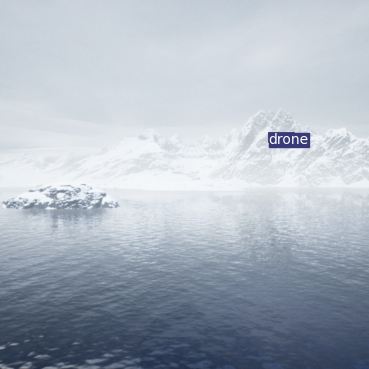
\includegraphics[width=\textwidth]{01640.png}
	\end{subfigure}
	\hfill
	\begin{subfigure}[b]{0.4\textwidth}
		\centering
		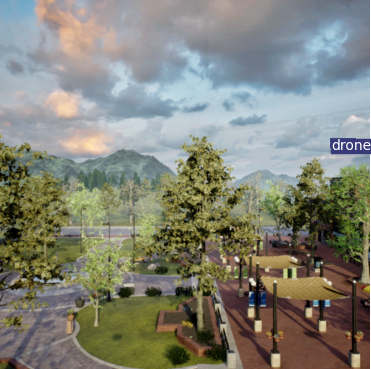
\includegraphics[width=\textwidth]{02002.png}
	\end{subfigure}
	\hfill
	\begin{subfigure}[b]{0.4\textwidth}
		\centering
		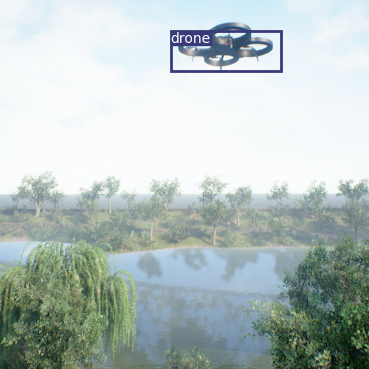
\includegraphics[width=\textwidth]{02167.png}
	\end{subfigure}
	\hfill
	\begin{subfigure}[b]{0.4\textwidth}
		\centering
		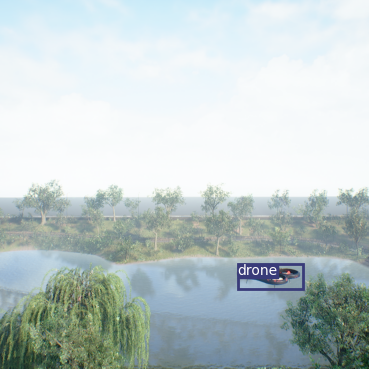
\includegraphics[width=\textwidth]{02665.png}
	\end{subfigure}
	\caption{Sample YOLOv3 outputs.}
\end{figure}
\chapter{Results}
After the training completed the different metrics on the validation dataset were compared. These metrics include:
\begin{itemize}
	\item Precision,
	\item Recall,
	\item Intersection over Union,
	\item Mean Average Precision (mAP).
\end{itemize}
These metrics are given by the following formulas:
\begin{equation}
\begin{aligned}
	Precision &= \frac{\text{True Positives}}{\text{True Positives} + \text{False Positives}},\\
	Recall &= \frac{\text{True Positives}}{\text{True Positives} + \text{False Negatives}},\\
	IoU &= \frac{\text{Area of overlap of two bounding boxes}}{\text{Area of union of two bounding boxes}},\\
	mAP &= \frac{1}{N}\sum^N_{i=1}AP_i.
\end{aligned}
\end{equation}
where:
\begin{itemize}
	\item $N$ is number of classes,
	\item $AP$ is Average Precision, an area under the Precision Recall curve.
\end{itemize}
In this case the dataset consisted of only one class, which is drone. Therefore $mAP=AP$.
\begin{figure}[h]
	\centering
	\begin{subfigure}[b]{0.49\textwidth}
		\centering
		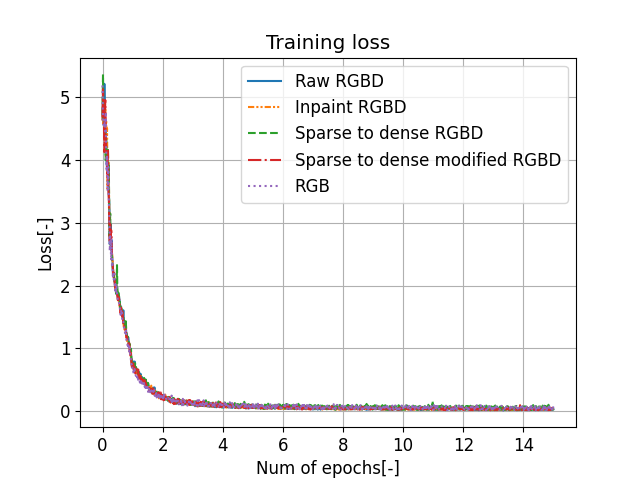
\includegraphics[width=\textwidth]{train_loss.png}
	\end{subfigure}
	\hfill
	\begin{subfigure}[b]{0.49\textwidth}
		\centering
		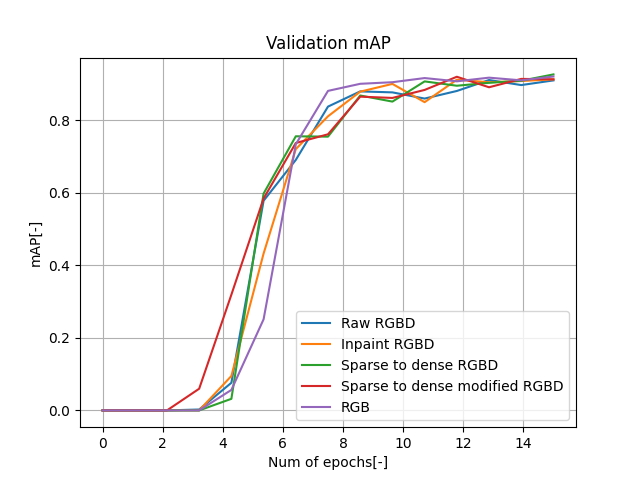
\includegraphics[width=\textwidth]{validation_mAP.png}
	\end{subfigure}
	\caption{Training results}
\end{figure}
For the training results validation mAP followed the training loss and started converging after around 8th epoch. It fully stopped rising after 12th epoch. Considering this the chosen weights ensured that the network does not overfit the training and validating dataset. For each input following weights were chosen:
\begin{table}[h]
	\begin{tabular}{|c|c|c|c|c|c|}
		\hline
		& \begin{tabular}[c]{@{}c@{}}Raw\\ RGBD\end{tabular} & \begin{tabular}[c]{@{}c@{}}Inpaint\\ RGBD\end{tabular} & \begin{tabular}[c]{@{}c@{}}Sparse to dense\\ RGBD\end{tabular} & \begin{tabular}[c]{@{}c@{}}Sparse to dense\\ modified RGBD\end{tabular} & RGB \\ \hline
		Weigths{[}epoch{]} & 9                                                  & 9                                                      & 11                                                             & 12                                                                      & 8   \\ \hline
	\end{tabular}
	\caption{Chosen weights.}
\end{table}\\
After the weights were chosen the network was validated on the test dataset. The confidence threshold was chosen to be $0.2$. The results were as following:
\begin{table}[h]
	\begin{tabular}{|c|c|c|c|c|c|}
		\hline
		Results   & \begin{tabular}[c]{@{}c@{}}Raw\\ RGBD\end{tabular} & \begin{tabular}[c]{@{}c@{}}Inpaint\\ RGBD\end{tabular} & \begin{tabular}[c]{@{}c@{}}Sparse to dense\\ RGBD\end{tabular} & \begin{tabular}[c]{@{}c@{}}Sparse to dense\\ modified RGBD\end{tabular} & RGB  \\ \hline
		mAP       & \textbf{0.48}                                      & 0.46                                                   & 0.36                                                           & 0.43                                                                    & 0.41 \\ \hline
		Precision & 0.59                                               & 0.89                                                   & \textbf{0.92}                                                  & 0.60                                                                    & 0.79 \\ \hline
		Recall    & \textbf{0.53}                                      & 0.48                                                   & 0.37                                                           & 0.48                                                                    & 0.48 \\ \hline
		IoU       & 0.79                                               & \textbf{0.84}                                          & \textbf{0.84}                                                  & 0.83                                                                    & 0.83 \\ \hline
	\end{tabular}
	\caption{Testing results}
\end{table}\\
\pagebreak
\begin{figure}[h!]
	\centering
	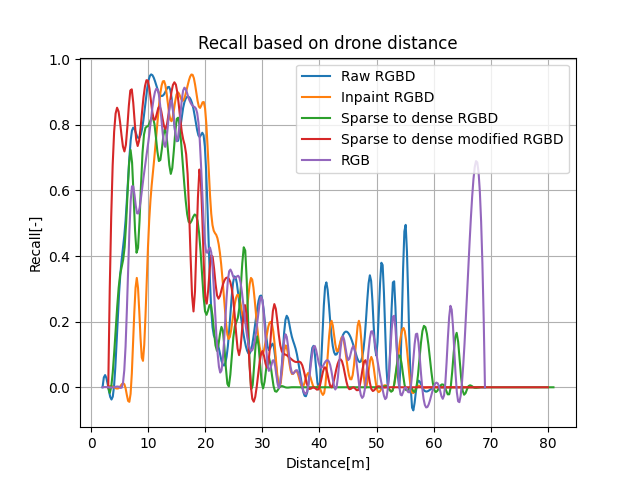
\includegraphics[width=\textwidth]{recall_distance.png}
	\caption{Recall based on distance of the drone.} \label{fig:recall_distance}
\end{figure}\\
From the results Raw RGBD offers the best improvement in terms of mAP by 7\%. Every method except unmodified Sparse to dense offers some improvement in terms of mAP. In terms of precision unmodified Sparse to dense and Inpaint offer improvement over RGB by 13\% and 10\% respectively. Other methods namely Raw RGBD and modified Sparse to dense offer a decrease of 20\% and 19\% respectively. When it comes to recall not a big improvement is made. The best method is Raw RGBD with an increase of 5\% in comparison to RGB. Unmodified Sparse to dense suffers a decrease of 11\% in comparison to RGB, while the remaining methods are unchanged. This can be observed in \autoref{fig:recall_distance} where all methods perform the best in range from 4 to 19 meters reaching maximum recall of around 0.95. Modified Sparse to dense offers highest recall in around 4 meters but starts to fall after 18 meters. Raw RGBD shows a few spikes in range from around 48 to 55 meters, the highest reaching 0.5 recall. RGB shows spike at around 67 meters with recall of around 0.7. In terms of IoU all methods perform very similarly with best performing methods Inpaint RGBD and unmodified Sparse to dense showing improvement of 1\%.
\pagebreak
\begin{table}[h]
	\begin{tabular}{|c|c|c|c|c|c|}
		\hline
		Speed       & \begin{tabular}[c]{@{}c@{}}Raw\\ RGBD\end{tabular} & \begin{tabular}[c]{@{}c@{}}Inpaint\\ RGBD\end{tabular} & \begin{tabular}[c]{@{}c@{}}Sparse to dense\\ RGBD\end{tabular} & \begin{tabular}[c]{@{}c@{}}Sparse to dense\\ modified RGBD\end{tabular} & RGB             \\ \hline
		time{[}s{]} & 0.0610                                             & 0.5424                                                 & 0.0669                                                         & 0.0759                                                                  & \textbf{0.0390} \\ \hline
	\end{tabular}
	\caption{Inference speeds of all methods.}
\end{table}
The inference speed was measured as a sum of all processing times that needed to be done before the detection was made simulating real-life application. From the results the 4th channel depth input almost doubles the inference time of YOLOv3, while Sparse to dense network alone performs quite fast. The longest time for inference belongs to Inpaint RGBD method with 0.5424 seconds. 
\bibliographystyle{amsalpha}
\bibliography{ctutest}
\end{document}
